\documentclass[titlepage,a4paper]{jsarticle}
\usepackage{../sty/import}% 各種パッケージインポート
\usepackage{../sty/title}% タイトルページの変更

%% タイトルページの変数
% レポートタイトル
\title{環境経済学期末試験}
% 提出日
\expdate{\today}
% 科目名
\subject{環境経済学}
% 分野
\class{情報経営システム工学分野}
% 学年
\grade{B3}
% 学籍番号
\mynumber{24336488}
% 記述者
\author{本間三暉}

\begin{document}
% titleページ作成
\maketitle
\section{記述問題}
\subsection*{国際交渉の結果、ある国が二酸化炭素排出量をXトン削減する義務を負うことになった。
  そこで、 図\ref{環境図}のとおり、政府は、Raの限界削減コスト曲線を持つ企業Aに、Xaトンの削減量を、Rbの限界削減 コスト曲線を持つ企業Bに、Xbトンの削減量を割り当てたとする。
  ただし、X=Xa+Xbと仮定する。}
\begin{figure}[H]
  \centering
  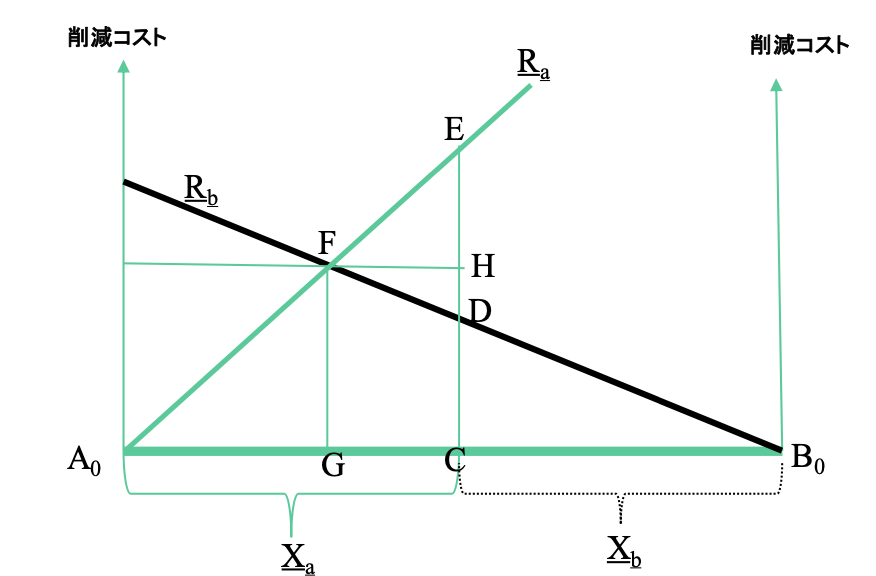
\includegraphics[width=12cm]{img/env.png}
  \caption{環境図}
  \label{環境図}
\end{figure}

\subsection{二酸化炭素削減量取引を許さない場合の削減コストを求めよ。}\label{問一}
図\ref{環境図}より,企業Aの削減コストが$\triangle A_0CE$,企業Bの削減コストが$\triangle B_0CD$なので,
二酸化炭素削減量取引を許さない場合の全体の削減コストは式\eqref{1:削減コスト}に示す通り,$\square A_0EDB_0$となる.
\begin{align}
  \triangle A_0CE + \triangle B_0CD = \square A_0EDB_0 \label{1:削減コスト}
\end{align}

\subsection{二酸化炭素削減量取引を許す場合の削減コストを求めよ。}\label{問二}
図\ref{環境図}より,企業Aの削減コストが$\triangle A_0FG$,企業Bの削減コストが$\triangle B_0FG$なので,
二酸化炭素削減量取引を許す場合の全体の削減コストは式\eqref{2:削減コスト}に示す通り,$\triangle A_0FB_0$となる.
\begin{align}
  \triangle A_0FG + \triangle B_0FG = \triangle A_0FB_0 \label{2:削減コスト}
\end{align}

\subsection{二酸化炭素削減量取引を許す場合と許さない場合の削減コストを比較せよ。}
図\ref{環境図}と節\ref{問一},\ref{問二}より,炭素削減量取引を許す場合は許さない場合に比べ式\eqref{3:差分}に示す通り,コストは$EFD$減少する.
\begin{align}
  \square A_0EDB_0 - \triangle A_0FB_0 = \triangle DEF\label{3:差分}
\end{align}
次に,$CG$分がB社からA社に単品価格$H$で販売されるので,販売額は$\square FHCG$となる.
この取引からB社は,販売収入$\square FHCG$から生産コスト$\square FDCG$を差し引いた$\triangle HDF$分の利益を上げる.
また,A社は取引を通じて,$\square GCEF$分の生産コストを削減し,そのうちの$\square FHGC$分を取引代金としてB社に支払うが,
残りの$\triangle FEH$分は避けられたコストであり,利益増加分に等しい.
よって,両方の会社にとって利益があり,取引することで生産コストを$EFD$削減することができる.

\subsection{二酸化炭素削減量取引を許す場合の、取引量、取引価格を求めよ。}
取引量は$R_a$と$R_b$の交点から削減量までの部分に相当するので$CG$,取引価格は$R_a$と$R_b$の交点までの高さに相当するので$FG$となる.

\section{レポート課題}
\renewcommand{\thesubsection}{\arabic{subsection}}
\subsection*{道路輸送部門の脱炭素化を実現するために、自動車の電動化が必要不可欠である。
  自動車電動化の推進にどのような対策が必要か、ZEV(Zero Emission Vehicle)目標規制・クレジット取引制度をどう位置づけるか等について、検討せよ。}
\subsection{自動車電動化の必要性}
道路輸送部門の脱炭素化は,地球温暖化対策の中でも重要な課題である.
内燃機関車両(ICEV)の排出する二酸化炭素($CO_2$)は,温室効果ガスの主要な原因の一つである.
これを削減するためには,電動化が必要不可欠である.
電動自動車(EV)は走行時に$CO_2$を排出せず,再生可能エネルギーで充電することで,エネルギー全体のカーボンフットプリントを大幅に低減できる.

\subsection{電動化推進のための対策}
電動化を促進するためには,以下のような政策や対策が必要である.
\begin{enumerate}
  \item インフラ整備: 充電ステーションの整備はEVの普及に不可欠である.充電時間の短縮,充電ポイントの拡充,スマートグリッド技術の導入などが求められる.
  \item 経済的インセンティブ: EV購入時の補助金,税制優遇措置,駐車料金の減免など,経済的なメリットを提供することで消費者のEV購入を促進する.
  \item 研究開発の支援: 電池技術や再生可能エネルギーの効率向上など,EVに関連する技術開発を支援するための資金提供が重要である.
  \item 教育と啓発活動: EVのメリットや使用方法に関する情報提供を通じて,消費者の理解を深め,EVの普及を促す.
\end{enumerate}
\subsection{ZEV目標規制とクレジット取引制度}
ZEV目標規制やクレジット取引制度は,電動化推進のための重要な政策手段である.
\begin{enumerate}
  \item ZEV目標規制: 各国や地域がゼロエミッション車(ZEV)の販売目標を設定し,自動車メーカーに一定割合のZEVを販売することを義務付ける制度である.
        これにより,自動車メーカーはZEVの開発・販売に注力せざるを得なくなる.
  \item クレジット取引制度: 自動車メーカーがZEVの販売目標を達成するために,他のメーカーとクレジットを取引できる制度である.
        目標を達成したメーカーは余ったクレジットを他のメーカーに売却でき,目標未達のメーカーはクレジットを購入して目標を達成することができる.
        この制度は,市場メカニズムを利用して効率的にZEVの普及を促進する.
\end{enumerate}
\subsection{具体例と考察}
例えば,カリフォルニア州のZEV規制は,2035年までに新車販売の100\%をZEVとする目標を掲げている.
このような先進的な取り組みが他の地域にも広がることで,グローバルなEV普及が進むと期待される.

さらに,クレジット取引制度が導入されることで,メーカー間の競争が激化し,技術革新が促進される.
これは,より高性能で低価格のEVが市場に投入されるきっかけとなり,消費者にとってもメリットがある.
\subsection{日本での取り組み}
日本での取り組みとして,補助金について取り上げて考える.

日本での2023年の燃料別新車販売台数(普通乗用車)の割合を\ref{EV図}に示す\cite{EV}.
\begin{figure}[H]
  \centering
  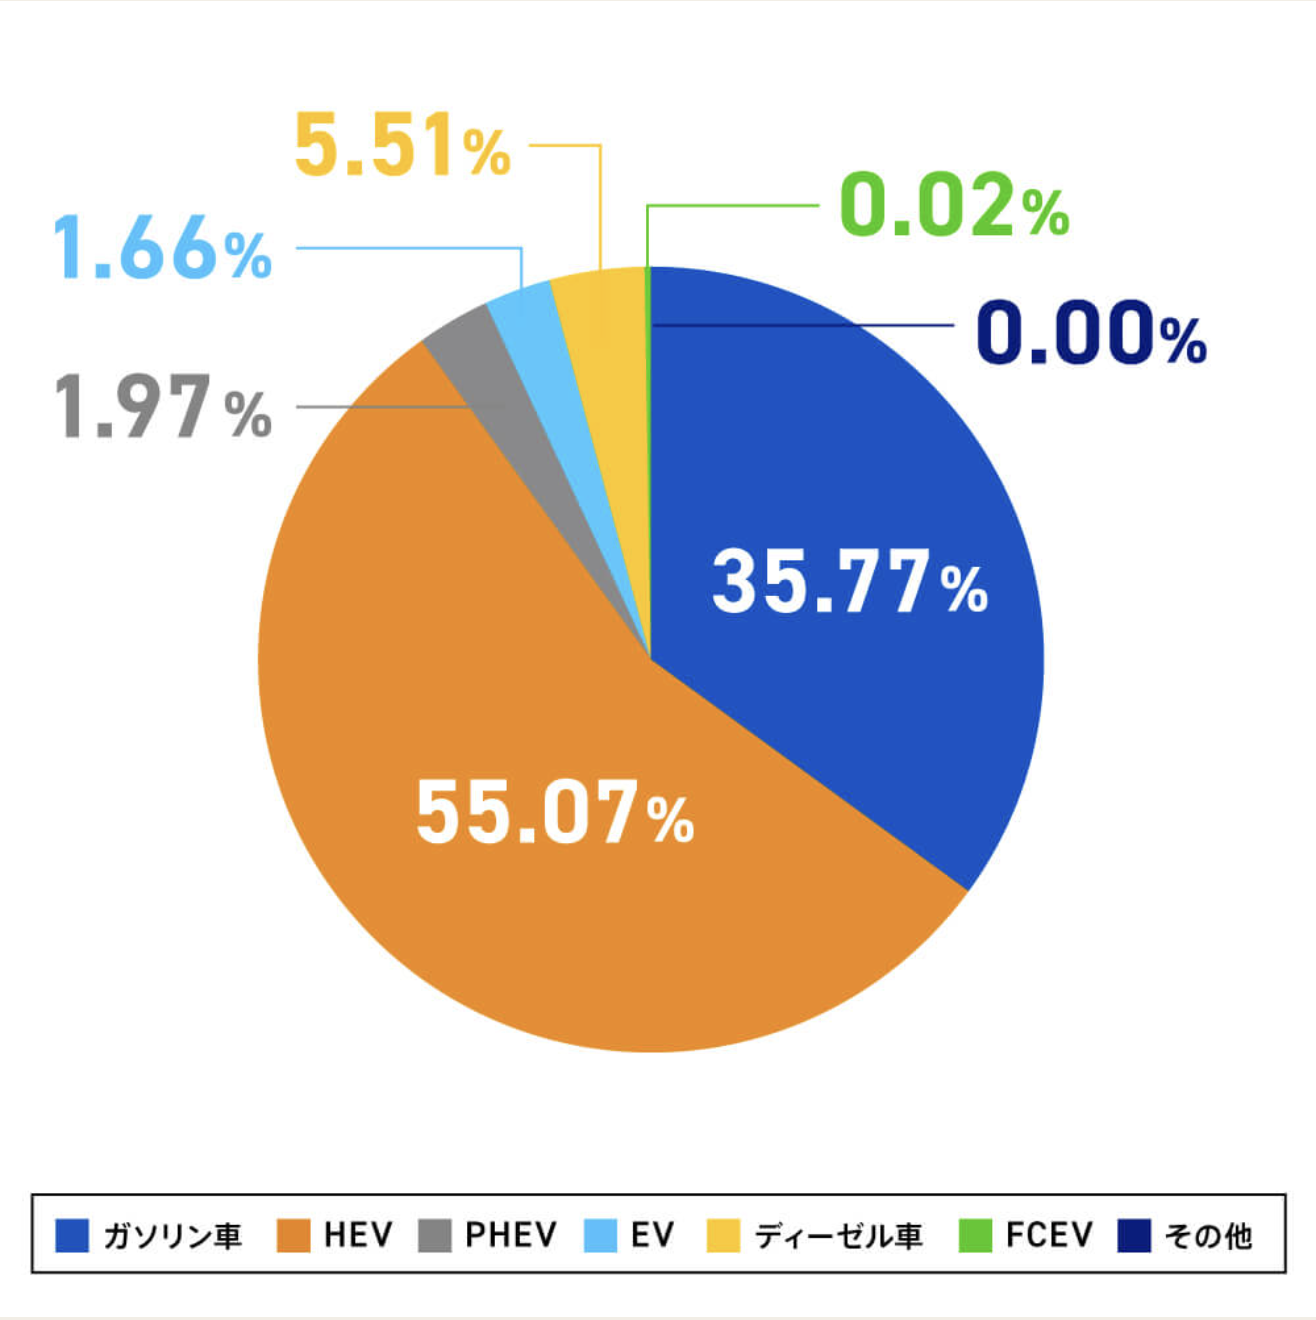
\includegraphics[width=0.8\textwidth]{img/2023EV.png}
  \caption{2023年の燃料別新車販売台数(普通乗用車)の割合}
  \label{EV図}
\end{figure}
普通乗用車の販売台数は265万1397台であったが,そのうちEVのシェア率は1.66\%とかなり低い.
これに関して,「価格が高い」,「充電ステーションが少ない」といった意見が主な理由となっている\cite{スタンド}.
これら問題を補助金を支給することで解決できると考えている.

また,この考えを補強する情報として,EV・PHEV月別販売台数・販売シェアの推移を図\ref{EVグラフ}に示す.
\begin{figure}[H]
  \centering
  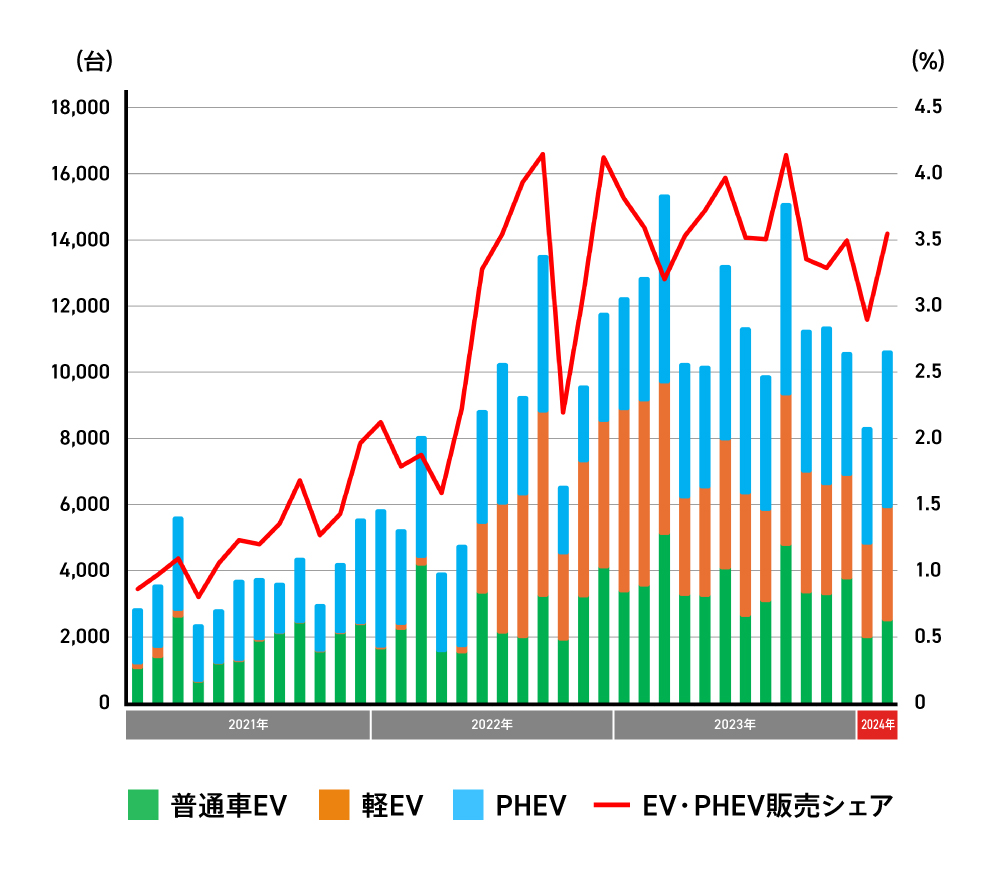
\includegraphics[width=0.8\textwidth]{img/EV_graph.jpeg}
  \caption{EV・PHEV月別販売台数・販売シェアの推移}
  \label{EVグラフ}
\end{figure}
これを見ると,2024年1・2月における普通乗用車のEVのシェアは約1.16\%(約4600台)となっており,2023年EVシェア率に比べ下がってしまっている.
これの原因として.2023年度の国のEV補助金が2月で一旦終了したことが影響していると考えられる.
\subsection{結論}
道路輸送部門の脱炭素化を実現するためには,電動化が避けて通れない道である.
インフラ整備,経済的インセンティブ,研究開発支援,教育・啓発活動といった総合的な対策が求められる.
また,ZEV目標規制やクレジット取引制度は,これらの対策を支える重要な政策手段である.
これらを効果的に組み合わせることで,持続可能な未来に向けた一歩を踏み出すことができる.
% 参考文献
\begin{thebibliography}{99}
  \bibitem{a}Homepage | California Air Resources Board\url{https://ww2.arb.ca.gov/}
  \bibitem{aa}IEA | International Energy Agency\url{https://www.iea.org/}
  \bibitem{EV}【2024年最新】EVの普及率はどのくらい?日本と世界のEV事情を解説 - EV DAYS | 東京電力エナジーパートナー\\
  \url{https://evdays.tepco.co.jp/entry/2021/09/28/000020}
  \bibitem{スタンド}株式会社マイナビ.``電気自動車を買わない理由は?2位は「充電ステーションが少ない」''.\\
  \url{https://news.mynavi.jp/article/20220830-2438191/}
\end{thebibliography}
参考文献は2024-7/30に閲覧
\end{document}